
%!TEX root = ../DSPP.tex
\documentclass[10pt, a4paper]{scrreprt}
\usepackage[ngerman]{babel}
\usepackage[T1]{fontenc} % needed to display the pipe symbol correct
\usepackage[utf8x]{inputenc}
\usepackage{cite}
\usepackage[colorlinks]{hyperref}
\usepackage{color}
\usepackage{colortbl}
\usepackage{graphicx}
\usepackage{graphics}
\usepackage{mathtools}
\usepackage{tikz} % Charts
\usepackage{amsmath}
\usepackage{tabularx}
\usepackage{caption}
\usepackage{xcolor}
\usepackage[bottom]{footmisc}
\usepackage{listings}
\usepackage{url}
\usepackage{hyperref}
\usepackage{tocloft}
\usepackage{moreverb}
\usepackage{supertabular}
\usepackage[tracking,kerning,spacing]{microtype} 
\usepackage{lmodern}                % optimierte Standard-Schrift für nicht-englische Texte
\usepackage[section]{placeins}      % Gleitobjekte dürfen jetzt sections nicht mehr verlassen
% Optionen für die PDF Ausgabe und Hyperlinks
\hypersetup{
    pdftitle={Distributed Systems and Parallel Processing},
    pdfauthor={Julian Vollmer, Philip Stewart},
    pdfsubject={openCL},
    pdfcreator={Julian Vollmer},
    colorlinks=true,    % false: boxed links; true: colored links
    linkcolor=black,    % color of internal links
    citecolor=black,    % color of links to bibliography
    filecolor=black,    % color of file links
    urlcolor=black      % color of external links
}

\lstset{
language=C++, % oder C++, Pascal, {[77]Fortran}, ...
numbers=left, % Position der Zeilennummerierung
firstnumber=auto, % Erste Zeilennummer
basicstyle=\ttfamily, % Textgröße des Standardtexts
keywordstyle=\ttfamily\color{darkgviolett}, % Formattierung Schlüsselwörter
commentstyle=\ttfamily\color{darkgreen}, % Formattierung Kommentar
stringstyle=\ttfamily\color{blue}, % Formattierung Strings
numberstyle=\tiny, % Textgröße der Zeilennummern
stepnumber=1, % Angezeigte Zeilennummern
numbersep=5pt, % Abstand zw. Zeilennummern und Code
aboveskip=15pt, % Abstand oberhalb des Codes
belowskip=11pt, % Abstand unterhalb des Codes
captionpos=b, % Position der Überschrift
xleftmargin=10pt, % Linke Einrückung
frame=single, % Rahmentyp
breaklines=true, % Umbruch langer Zeilen
showstringspaces=false % Spezielles Zeichen für Leerzeichen
}

\newenvironment{mylisting}
{\begin{list}{}{\setlength{\leftmargin}{1em}}\item\scriptsize\bfseries}
{\end{list}}

\newenvironment{mytinylisting}
{\begin{list}{}{\setlength{\leftmargin}{1em}}\item\tiny\bfseries}
{\end{list}}

%\usepackage{glossaries}
%\newglossaryentry{dotnetkomponenten}{
 	name=.NET-Komponenten*,
	description={Die Begriffe CLR-Komponente, .NET-Komponente und CLI-Komponente sind synonyme Bezeichnungen für eine Softwarekomponente im .NET Framework/der Common Language Infrastructure}
}
\newglossaryentry{zeiger}{
 	name=Zeiger*,
	description={Mit Zeiger (auch engl. Pointer) wird in der Informatik ein Wert bezeichnet, welcher auf eine Speicheraddresse verweist}
}
\newglossaryentry{delegaten}{
 	name=Delegaten*,
	description={Delegaten sind in C und C++ als Funktionszeiger bekannt, bieten aber in eine größernen Funktionsumfang und arbeiten mit Signaturen}
}
\newglossaryentry{cilcode}{
 	name=CIL-Zwischencode*,
	description=Common Intermediate Language (CIL) (teilweise auch nur Intermediate Language (IL)) ist eine Zwischensprache{,} in die alle Programme der Common Language Infrastructure uebersetzt werden. CIL ist eine objektorientierte Assemblersprache und ist vollstaendig stackbasiert
}
\newglossaryentry{wrapper}{
 	name=Wrapper*,
	description=Ein Wrapper ist eine Software{,}  welche eine andere Software umhuellt um die Funktionalitaet der umhuellten Software bereitzustellen
}
\newglossaryentry{adonet}{
 	name=ADO.NET*,
	description=ADO.NET ist ein Teil der von Microsoft entwickelten .NET-Plattform. Es handelt sich um eine Sammlung von Klassen{,} die den Zugriff auf relationale Datenbanken gewährleisten
}
\newglossaryentry{kompilierung}{
 	name=Kompilierung*,
	description=Unter Kompilierung (auch Compilierung oder Übersetzung oder Wandlung) versteht man in der EDV die Anwendung eines Compilers auf den Quelltext eines Computerprogramms. Dabei wird das in einer Quellsprache geschriebene Programm in ein semantisch äquivalentes Programm in der Zielsprache übersetzt.
}
\newglossaryentry{deklarativ}{
 	name=deklarativ*,
	description=Deklarative Programmiersprachen gestatten eine Beschreibung des Problems in der Form{,} dass die relevanten Sachverhalte und die Beziehungen zwischen diesen angegeben werden. Die als Ergebnis gewünschten Sachverhalte werden aus der Problembeschreibung automatisch abgeleitet{,} sofern ein Lösungsweg gefunden werden kann \footnote{\url{http://wirtschaftslexikon.gabler.de/Archiv/57318/programmiersprache-v7.html}}
}
\newglossaryentry{CommonLanguageRuntime}{
 	name=Common Language Runtime*,
	description=Die Common Language Runtime ist die Laufzeitumgebung von .NET und stellt  den Interpreter für den Zwischencode dar \footnote{\url{http://wirtschaftslexikon.gabler.de/Archiv/57318/programmiersprache-v7.html}}
}

\newglossaryentry{ecma}{
 	name=ECMA*,
	description=Ecma International (Ecma) ist eine private{,} internationale Normungsorganisation zur Normung von Informations- und Kommunikationssystemen und Unterhaltungselektronik \footnote{\url{http://de.wikipedia.org/wiki/Ecma_International}}
}

\newglossaryentry{ssd}{
 	name=SSD*,
	description={Solid-State-Disks speichern die Daten, gegenüber Festplatten, welche auf magnetisierbaren Oberfläche die Daten ablegen, auf Flashspeichern}
}

\newglossaryentry{srgb}{
 	name=sRGB*,
	description=Standard Red-Green-Blue{,} zu deutsch{,} Standard Rot-Grün-Blau
}

\newglossaryentry{ConsumerTablets}{
 	name=Consumer-Tablets*,
	description=Consumer-Tablets sind von der Leistung her{,} hauptsächlich für das Komsumieren von Medien hergestellt.
}
\newglossaryentry{kompiler}{
 	name=Kompiler*,
	description=Ein Compiler ist ein Programm{,} mit dem symbolische Programmiersprachen der zweiten bis vierten Generation in lauffähige Maschinensprachen umgesetzt werden \footnote{\url{http://www.itwissen.info/definition/lexikon/Compiler-compiler.html}}
}

\newglossaryentry{delphi}{
 	name=Delphi*,
	description=Delphi ist zum einen der Name einer vom Unternehmen Borland entwickelten objektorientierten Programmiersprache{,} die ursprünglich aus der von Niklaus Wirth erstellten Programmiersprache Pascal hervorgegangen ist \footnote{\url{http://de.wikipedia.org/wiki/Embarcadero_Delphi}}
}
\newglossaryentry{kombiaudio}{
 	name=kombinierter Audio-Port*,
	description={Ein kombinierter Audio-Port benutzt einen Anschluss für Microfone(Line-In) und Kopfhörer(Line-Out), diese Technik ist bekannt aus Smartphones, und etablierte sich bei Geräten die klein gehalten werden sollen}
}





%\makeglossaries

\DeclareCaptionFont{white}{\color{white}}
\DeclareCaptionFormat{listing}{\colorbox{gray}{\parbox{\textwidth}{#1#2#3}}}
\captionsetup[lstlisting]{format=listing,labelfont=white,textfont=white}
\parindent0pt 			% Nicht einrücken
\usepackage{geometry}	%\geometry{a4paper,left=30mm,right=30mm, top=20mm, bottom=20mm} 
\nonfrenchspacing
\pagestyle{headings}
\definecolor{darkblue}{rgb}{0,0,.5}
\hypersetup{colorlinks=true, breaklinks=true, linkcolor=darkblue, menucolor=darkblue,  urlcolor=darkblue}
\definecolor{tblUeberschriftFarbe}{rgb}{0.8,0.8,0.8}
\cellcolor{tblUeberschriftFarbe}

\renewcommand{\cftfigpresnum}{Abb. } % Name vor der Nr. 
\renewcommand{\cftfigaftersnum}{:} % Doppelpunkt nach der Nr.
\settowidth{\cftfignumwidth}{Abb. 100\quad}

\title{Distributed Systems and Parallel Processing - \textbf{"`???"'}}
\author{Julian Vollmer}
\date{\today}

\begin{document}

\newcommand{\thema} {Datenanalyse zur Erkennung des Händigkeitsprofil bei Kindern}


\newcommand{\dig} {dig-TEMA}
\newcommand {\digcpl} {Entwicklung eines digitalen Test- und Evaluierungssystems für manuelle Aktionen}

\newcommand{\ifaf} {IFAF}
\newcommand{\ifafcpl} {Institut für angewandte Forschung Berlin e.V.}

\newcommand{\ash} {ASH}
\newcommand{\ashcpl} {Alice Salomon Hochschule Berlin}

\newcommand{\htw} {HTW}
\newcommand{\htwcpl} {Hochschule für Technik und Wirtschaft Berlin}

\newcommand{\tabletname} {Asus Eee Slate EP121}
\newcommand{\progname} {Handanalyse}
\newcommand{\prognamecpl} {\glqq{}Handanlyse\grqq{}}
\newcommand{\logger} {Humotion Datenlogger}
\newcommand{\emgu} {EmguCV}

\newcommand{\forte} {Prof. Dr. Fortenbacher}
\newcommand{\kraus} {Prof. Dr. Elke Kraus}
\newcommand{\woge} {Sebastian Woge}
\newcommand{\gaertner} {Prof. Dr. Dipl.-Ing. Hendrik Gärtner}


\newcommand{\magnet} {Magnetfeldsensor}
\newcommand{\gyro} {Gyroskop}
\newcommand{\beschleunigung} {Beschleunigungssensor}

\newcommand{\kinectsdk} {KinectSDK}
\newcommand{\kinect} {Microsoft Kinect}

\newcommand{\humotion} {Humotion GmbH}

%!TEX root = ../DSPP.tex
\begin{abstract}

\Large
\begin{center}

\includegraphics[scale=1.0]{./daten/HTW.jpg}\\

\vspace{30pt}

{\huge ???}\\
\textit{"`???"'}\\


\vspace{30pt}
Sommersemester 2013
\vspace{10pt}

\end{center}


\vspace{200pt}

\begin{flushleft}
Philip Stewart (526571)\\
Julian Vollmer (525904)\\

\vspace{20pt}

Fachbereich 4\\
Master Angewandte Informatik\\
Distributed Systems and Parallel Processing\\
\vspace{10pt}

\textbf{Betreuer:}\\
Sebastian Bauer\\



\end{flushleft}
\end{abstract}


%\newpage
%\input{./chapter/00_Vorwort}

\newpage

\hypersetup{linkcolor=black}

\setcounter{secnumdepth}{5} 
\setcounter{tocdepth}{5} 
\newgeometry{left=3cm,bottom=0.1cm}
\tableofcontents
\restoregeometry
\newpage

\chapter{Einleitung}
%!TEX root = ../DSPP.tex
\section{Hintergrund}
Motivation dieser Arbeit ist der Kurs \glqq{}M31.2 Distributed Systems and Parallel Processing\grqq{} im Sommersemester 2013 welcher vom Dozenten Herr Sebastian Bauer durchgeführt wurde. 
\section{Zielstellung}
Ziel dieser Arbeit ist es den küzesten Pfad zwischen 2 Punkten zu bestimmen. Dieses Problem kann efektiv mit dem Dijkstra Algorithmus gelöst werden. Im Rahmen des beiliegenden Projektes wird versucht diesen Algorithmus zu paralellisieren und dadurch einen Speedup \footnote{\url{http://de.wikipedia.org/wiki/Speedup}} zu erreichen.


\begin{figure}
  \centering
  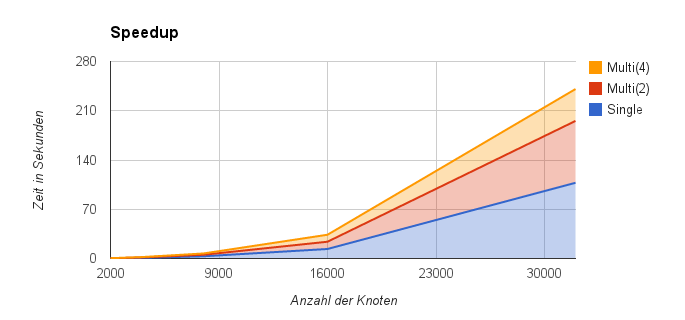
\includegraphics[width=0.8\textwidth]{./daten/speedup_openmp.png}
  \caption{Speedup OpenMP}
  \label{speedup_openmp}
\end{figure}
\chapter{Dijkstra}
%!TEX root = ../DSPP.tex
\section{Wie funktioniert er}
\chapter{Ablaufplan und Eckdaten}
%!TEX root = ../DSPP.tex
\section{Wie läuft sein Performance Test ab}

\begin{itemize}
	\item Knoten werden zufällig erzeugt
	\item Knotenanzahl wird um 2000 Knoten erhöht
\end{itemize}

\section{Eckdaten}
Es gibt zu einer wahrscheinlichkeit von 0.1\% ein Verbindung zwischen 2 Punkten.
\begin{verbatim} 
void ShortPath::init_random_distances(){
    ...
	if((liefere_ganze_zufallszahl(0,1000)%1000)==0){
	    it->add_distances_to_other(0);    
	}
	else{
	        it->add_distances_to_other(liefere_ganze_zufallszahl(1,250));    
	    }
    ...
} 

\end{verbatim} 


\section{Speedup-Berechnung}
hier die Speedup-Berechnung.
\chapter{User Interface Desgin}
%!TEX root = ../DSPP.tex

\begin{figure}
  \centering
  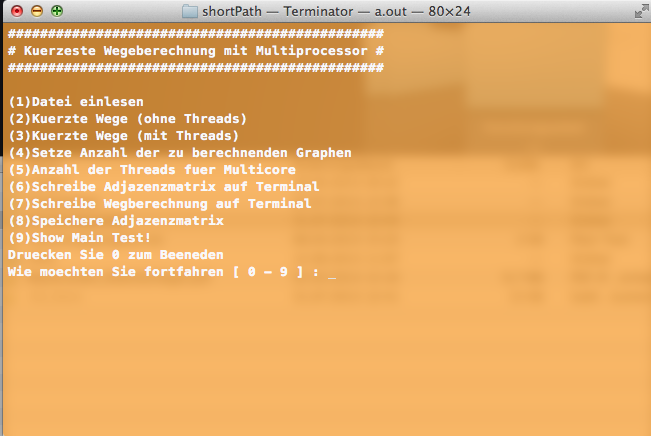
\includegraphics[width=0.8\textwidth]{./daten/ui_design.png}
  \caption{User Interface}
  \label{ui_design}
\end{figure}
\chapter{User Interface Desgin}
%!TEX root = ../DSPP.tex

\section{Abgabeinhalt}
Die Abgabe erfolgte Elektronisch in Form einer Zip-Datei. Folgende Informationen waren in dieser Zip-Datei enthalten 
\begin{itemize}
	\item Zwischenpräsentation
	\item Quellcode 
	\item Dokumentation (Doxygen)
	\item Dokumentation (dieses Dokument)

\end{itemize}

\section{Programm}

\section{Quelltextdokumtation}

\section{Zwischenstandspräsentation}
Die Zwischenpräsentation ist zu finden unter \url{http://de.slideshare.net/julianvollmer/distributed-systems-and-parallel-processing} 
\section{Kontakt}
Julian Vollmer
Maximilianstraße 25
10317 Berlin
julianvollmer@gmail.com



%\bibliographystyle{plain}
%\bibliography{Museumstechnologien}

%\input{./chapter/998_Literatur}

\newpage
\listoffigures
\newpage
%\renewcommand{\glossaryname}{Glossar}
%\printglossary[title=Glossar,toctitle=Glossar,]

%\chapter*{Anhang}\markboth{Anhang}{Anhang}
%\input{./chapter/999_Anhang}
%\chapter*{Eigenst채ndigkeitserkl채rung}
%\input{./chapter/eigenstaendigkeit}
\end{document}